%%%%%%%%%%%%%%%%%%don't forget if needed %%%%%%%%%%%%%%%%%%%%%
%\section[toc version]{title version%
%              \sectionmark{head version}}
%\sectionmark{head version}
%%%%%%%%%%%%%%%%%%%%%%%%%%%%%%%%%%%%%%%%%%%%%%%%%%%%%%%%%%%%%%
\def\titcourt{Numerical simulation three dimensional configuration using FFDDM}
\def\titlong{Numerical simulation three dimensional configuration using FFDDM}
%%%%%%%%%%%%%%%%%%%%%%%%%%%%%%%%%%%%%%%%%%%%%%%%%%%%%%%%%%%%%%%%
\chapter[\titlong]{\titlong%
              \chaptermark{\titcourt}}
\chaptermark{\titcourt}
\label{chap-3D-SIMULATION}
%%%%%%%%%%%%%%%%%%%%%%%%%%%%%%%%%%%%%%%%%%%%%%%%%%%%%%%%%%%%%%%%
%%%%%%%%%%%%%%%%%%%%%%%%%%%%%%%%%%%%%%%%%%%%%%%%%%%%%%%%%%%%%%%%

We first focus on the capability of our code to deal with natural convection flow in enclosures without phase-change.
The richness of studies on internal natural convection flow indeed allows us to validate the Navier-Stokes-Boussinesq solver in the fluid part.
A large number of benchmark solutions exists in the literature for natural convection induced by temperature difference since it is central in a long list of engineering and geophysical systems
(circulations in building applications, double-wall insulations, solar collectors, etc.).
The influence of the geometric aspect ratio, the inclination, the heating orientation (if we heat from the side of from below), the $\Ray$ number have been widely studied.
It is indeed well-known that the heat transfer is completely different from tall enclosure or shallow enclosure limits. 
In one case, the heat transfer is dominated by conductive transfer (such as double-wall insulations) and in the second case the heat transfer is dominated by the presence of vertical layer.
In this chapter, we are interested in natural convection of fluid in a square cavity differentially heated from the vertical walls.
Along the heated wall, the fluid temperature rises and its density decreases. 
Due to the density decrease, the fluid rises up to the point where it reaches the cold wall, where the reverse process occurs. 
This two simultaneous opposing effects create a recirculation cell. In the center of the cell, a stationary zone can be observed.

We solve the system of eqs. (\ref{eq-qmvt}) - (\ref{eq-energ}) without the penalty term $A(\theta) \vec u$ in the momentum equation and the source term $\partial (CS)/\partial t$ in the energy equation.
Linear and non-linear expressions of the buoyancy force $f_B(T)$ in the Boussinesq approximation (\ref{eq-energie-enth-model}) are investigated, by simulating the natural convection of air and the natural convection of water.
Natural convection of water exhibits actually a non-linear variation of the density with a maximum value around $T=4^o C$ while linear variation is generally assumed for the natural convection of air in the Boussinesq approximation.

\section{Numerical simulation of the natural convection of air in a three-dimensional cavity using parallel agorithm}\label{sec: natconv-air-3D}

\subsection{Natural convection of air in differentially heated cube cavity}
We present in this section some 3D simulations using ffddm.

The Prandtl number is $0.71$ and three Rayleigh numbers are considered:  $\Ray=10^4$, $\Ray=10^5$, $\Ray=10^6$. The walls are rigid and impermeable. The vertical walls at $x=0$ and $x=1$ are isothermal and have different temperatures $T_h=0.5$ and $T_c=-0.5$ respectively. The remaining walls are considered adiabatic. % Figure \ref{fig-3Dmesh} b) shows the present three dimensional grid.
 
Our result were obtained for uniform grids of $  40 \times 40 \times 40$ and is compared with \cite{Wakashima-2004} who used a forth order finite difference method, with a vorticity-stream function formulation with different uniform meshes of  $120 \times 120 \times 120 \times 10$ grid nodes. 
This result obtained with sequential algorithm is also used to validate the 3D simulations using ffddm.

Fig. \ref{fig-3DT} shows the temperature field for each of the three Rayleigh numbers $\Ray = 10^4$, $\Ray = 10^5$, $\Ray = 10^6$, at the mid section (y=0.5).
On the left we display the numerical results of \cite{Wakashima-2004} and on the right ou results.
The comparison with the benchmark solution exhibits a fairly good agreement.

The parallel algorithm used with ffddm is compared with the sequential algorithm.
$\mathcal{L}_2$-norm and $\mathcal{L}_\infty$-norm of the velocity and the temperature are computed and reported in Tab. \ref{tab-T1} for Rayleigh number varying from $10^4$ to $10^6$.
The difference between both algorithm is of order of $10^{-6}$.
Moreover, we do not observe a large variation of the error when the number of subdomains is increased.
The number of subdomain vary from $28$ to $70$ for $1.8$ millions of unknown.

\begin{table}[!h]
	\begin{center}
		\begin{tabular}{|*{6}{c|}}
			\hline
			 Ra & nb proc                     & $||u||_{2}$                        & $||u||_{\infty}$                & $||T||_{2}$              & $||T||_{\infty}$\\ \hline \hline
			\multirow{4}{*}{$10^4$} & 28 & $1.12496 \cdot 10^{-6}$ & $3.1 \cdot 10^{-6}$ & $ 3.09966 \cdot 10^{-6} $ & $7 \cdot 10^{-6}$ \\% \hline
			\cline{2-6}
			& 42 & $1.53698 \cdot 10^{-6}$ & $5.1 \cdot 10^{-6}$ & $ 3.23352 \cdot 10^{-6} $ & $8 \cdot 10^{-6}$ \\ \cline{2-6} %\hline 
			& 56 & $1.55576 \cdot 10^{-6}$ & $5.1 \cdot 10^{-6}$ & $ 3.4342 \cdot 10^{-6} $ & $8 \cdot 10^{-6}$  \\ \cline{2-6} %\hline
			& 70 & $1.25622 \cdot 10^{-6}$ & $3.6 \cdot 10^{-6}$ & $ 3.56048 \cdot 10^{-6} $ & $8 \cdot 10^{-6}$ \\ \hline \hline
			\multirow{4}{*}{$10^5$} & 28 & $1.73254 \cdot 10^{-6}$ & $6.1 \cdot 10^{-6}$ & $ 2.40467 \cdot 10^{-6} $ & $7 \cdot 10^{-6}$ \\% \hline
			\cline{2-6}
			& 42 & $2.84973 \cdot 10^{-6}$ & $7.78 \cdot 10^{-6}$ & $ 3.53003 \cdot 10^{-6} $ & $9 \cdot 10^{-6}$ \\ \cline{2-6} %\hline 
			& 56 & $3.00832 \cdot 10^{-6}$ & $7.39 \cdot 10^{-6}$ & $ 4.17769 \cdot 10^{-6} $ & $1.1 \cdot 10^{-5}$  \\ \cline{2-6} %\hline
			& 70 & $3.68118 \cdot 10^{-6}$ & $9 \cdot 10^{-6}$ & $ 4.70846 \cdot 10^{-6} $ & $1.2 \cdot 10^{-5}$ \\ \hline \hline
			\multirow{4}{*}{$10^6$} & 28 & $6.61804 \cdot 10^{-6}$ & $1.826 \cdot 10^{-5}$ & $ 3.46504\cdot 10^{-6} $ & $1.1 \cdot 10^{-5}$ \\% \hline
			\cline{2-6}
			& 42 & $5.93966 \cdot 10^{-6}$ & $1.5 \cdot 10^{-5}$ & $ 3.98082 \cdot 10^{-6} $ & $1.2 \cdot 10^{-5}$ \\ \cline{2-6} %\hline 
			& 56 & $7.05144 \cdot 10^{-6}$ & $1.9247 \cdot 10^{-5}$ & $ 5.0044 \cdot 10^{-6} $ & $2 \cdot 10^{-5}$  \\ \cline{2-6} %\hline
			& 70 & $6.02152 \cdot 10^{-6}$ & $1.68 \cdot 10^{-5}$ & $ 4.50094 \cdot 10^{-6} $ & $1.8 \cdot 10^{-5}$ \\ \hline
		\end{tabular}
	\end{center}
	\caption {3D differentially heated cavity. Comparison between sequential and ffddm algorithm for uniform grids of $40 \times 40 \times 40$ }
	\label{tab-T1}
\end{table}


\begin{figure}%[!htbp]
\begin{minipage}{\linewidth}
\begin{center}
 {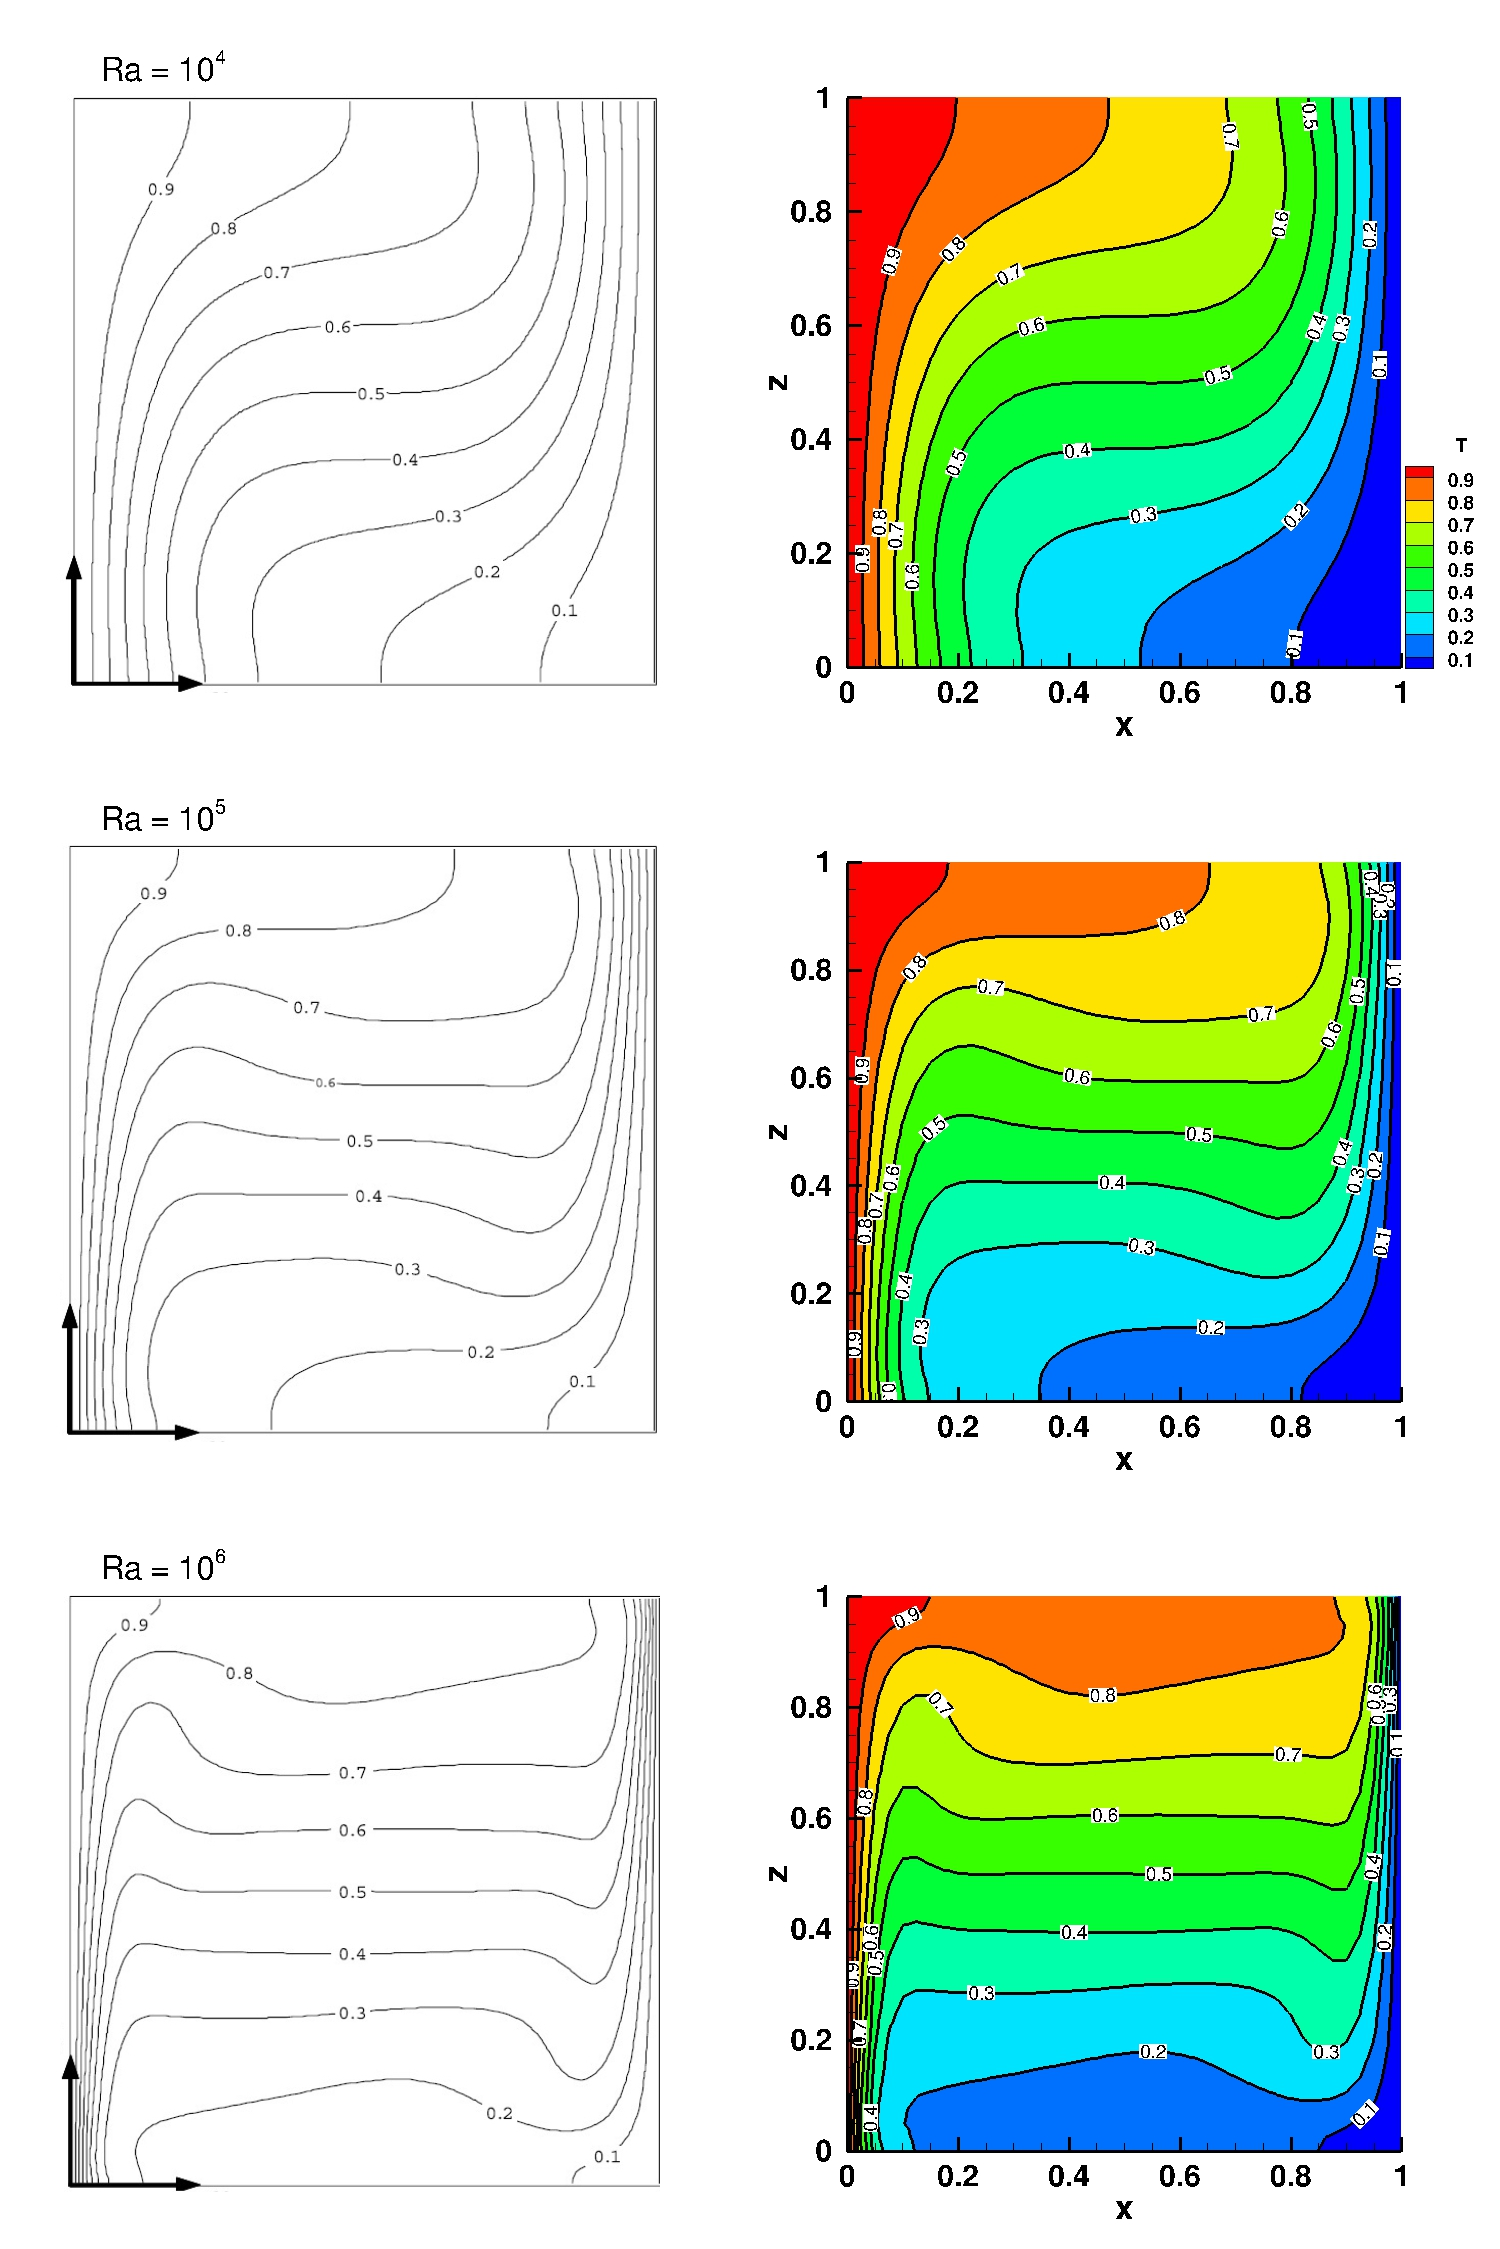
\includegraphics[width=\textwidth]{\figpath/Fig_cap_natconv/Validation_3D_seq_T1}}
\end{center}
\end{minipage}
\caption{3D differentially heated cavity. Temperature contours at the mid-plane of ($y=0.5$); comparison with the results of \cite{Wakashima-2004} (left images). }
\label{fig-3DT} 
\end{figure}

\subsection{Natural convection in a cube with an inner heated obstacle}\label{sub-OBSTACLE-3D}

The three-dimensional natural convection induced by a temperature difference between a cold outer cubic enclosure is investigated in this section.
Sequential and parallel computation using ffddm are carried out and compared together.

Different Rayleigh numbers varying in the range of $10^4 -10^6$ are considered. The temperature field for $Ra = 10^4$ is reported in Figure \ref{fig-obstacle-Ra1e4} and the Table \ref{tab-T2} shows the error between the sequential and the parallel computation.

\begin{figure}%[!htbp]
\begin{center}
\begin{minipage}{\linewidth}
 {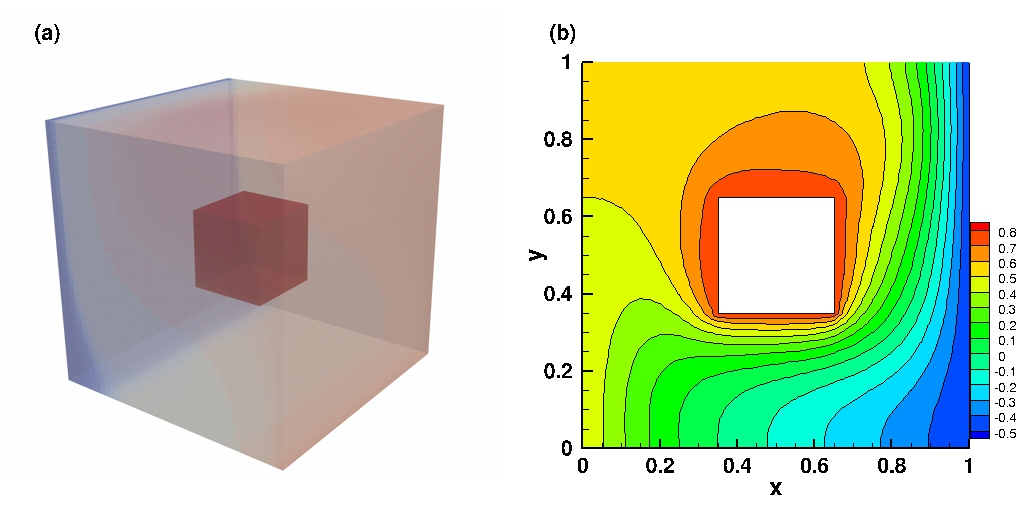
\includegraphics[width=0.98\textwidth]{\figpath/Fig_cap_natconv/3D_OBSTACLE_field}}
\end{minipage}
\end{center}
\caption{3D convection in a cube with an inner heated cube. Temperature fields for $Ra = 10^4$.}
\label{fig-obstacle-Ra1e4} 
\end{figure}

\begin{table}[!h]
	\begin{center}
		\begin{tabular}{|*{7}{c|}}
			\hline
			 Ra & nbseg & nb proc                     & $||u||_{2}$                        & $||u||_{\infty}$                & $||T||_{2}$              & $||T||_{\infty}$\\ \hline \hline
			\multirow{12}{*}{$10^4$} & \multirow{4}{*}{40} & 28 & $0.00087137$ & $0.0058298$ & $ 0.0022491 $ & $0.01592$ \\
			\cline{3-7}
			& & 42 & $0.000870796$ & $0.0058292$ & $ 0.00224866 $ & $0.015921$ \\ \cline{3-7} %\hline 
			& & 56 & $0.000870646$ & $0.0058293$ & $ 0.00224788 $ & $0.015921$  \\ \cline{3-7} %\hline
			& & 70 & $0.000870747$ & $0.0058286$ & $ 0.00224795 $ & $0.015921$ \\ \cline{2-7}
			 & \multirow{4}{*}{60} & 112 & $0.000785593$ & $0.0021$ & $ 0.000858912 $ & $0.010024$ \\% \hline
			\cline{3-7}
			& & 140 & $0.000783164$ & $0.002097$ & $ 0.000865668 $ & $0.010024$ \\ \cline{3-7} %\hline 
			& & 168 & $0.000779419$ & $0.002091$ & $ 0.000858384 $ & $0.010027$  \\ \cline{3-7} %\hline
			& & 196 & $0.000767662$ & $0.00209$ & $ 0.000864693 $ & $0.010019$ \\ \cline{2-7}
			 & \multirow{4}{*}{80} & 224 & $0.000637268$ & $0.001795$ & $ 0.000551538 $ & $0.001661$ \\% \hline
			\cline{3-7}
			& & 238 & $0.000152936$ & $0.000548$ & $ 0.000205031 $ & $0.000634$ \\ \cline{3-7} %\hline 
			& & 252 & $0.000239786$ & $0.000841$ & $ 0.000231648 $ & $0.000661$  \\ \cline{3-7} %\hline
			& & 266 & $0$ & $0$ & $ 0 $ & $0$ \\ \hline 
			\multirow{12}{*}{$10^5$}& \multirow{4}{*}{40} & 28 & $0.0011359$ & $0.0089746$ & $ 0.00401922 $ & $0.020067$ \\% \hline
			\cline{3-7}
			& & 42 & $0.00113742$ & $0.0089788$ & $ 0.00402103 $ & $0.020067$  \\ \cline{3-7} %\hline 
			& & 56 & $0.00113625$ & $0.0089768$ & $ 0.00402081 $ & $0.020063$   \\ \cline{3-7}%\hline
			& & 70 & $0.0011348$ & $0.0089726$ & $ 0.00401999 $ & $0.020065$  \\ \cline{2-7} %\hline
			 & \multirow{4}{*}{60} & 112 & $0.000765582$ & $0.0022345$ & $ 0.00166687 $ & $0.015296$ \\% \hline
			\cline{3-7}
			& & 140 & $0.000763449$ & $0.0022313$ & $ 0.00166143 $ & $0.015257$ \\ \cline{3-7} %\hline 
			& & 168 & $0.000763074$ & $0.0022176$ & $ 0.00166605 $ & $0.015284$  \\ \cline{3-7} %\hline
			& & 196 & $0.000760368$ & $0.0022093$ & $ 0.00167368 $ & $0.015299$ \\ \cline{2-7} 
			 & \multirow{4}{*}{80} & 224 & $0.00051462$ & $0.0016627$ & $ 0.000574467 $ & $0.001794$ \\% \hline
			\cline{3-7}
			& & 238 & $5.17443 \times 10^{-05}$ & $0.0001934$ & $ 0.00018074 $ & $0.0005666$ \\ \cline{3-7} %\hline 
			& & 252 & $8.68245 \times 10^{-05}$ & $0.000319$ & $ 8.11788 \times 10^{-05} $ & $0.000335$  \\ \cline{3-7} %\hline
			& & 266 & $0$ & $0$ & $ 0 $ & $0$ \\ \hline 

		\end{tabular}
	\end{center}
	\caption {3D convection in a cube with an inner heated cube. Comparison between sequential and ffddm algorithm for uniform grids of $40 \times 40 \times 40$ for $Ra = 10^4$ and $80 \times 80 \times 80$ for $Ra = 10^5$}
	\label{tab-T2}
\end{table}
